\documentclass[letterpaper]{article}
\usepackage[submission]{aaai2027}
\usepackage[hyphens]{url}
\usepackage{graphicx}
\urlstyle{rm}
\def\UrlFont{\rm}
\usepackage{natbib}
\usepackage{caption}
\usepackage{booktabs}
\frenchspacing
\pdfinfo{/TemplateVersion (2027.1)}
\setcounter{secnumdepth}{0}
\title{From Sycophantic Behavior to User Consequences:\\An Evidence Audit of a Literature Map}
\author{Anonymous Submission}
\affiliations{}

\begin{document}
\maketitle
\begin{abstract}
Identifying sycophantic model behavior does not establish its consequences for people. We examine how an existing literature map connects behavior definitions, evaluators, and outcomes, using descriptive analysis of 31 publication records and a focused full-text audit of three included empirical papers. The supplied coding marks system performance in 12 records, user opinion in 11, user action in eight, and user task performance in four. Fifteen records have at least one user outcome; only one is also marked for system performance. These are coding-coverage results, not verified prevalence estimates: the audit identifies unmarked measures and distinguishes perceived advice quality from recipient outcomes. Behavior--outcome intersections are uneven, but do not establish differences in harms across behavior types. The synthesis identifies a practical requirement for interpretable sycophancy evaluations: distinguish who judges an output, what the measure represents, and whether it observes a user consequence. Incomplete selection and coding provenance limits generalization beyond this corpus.
\end{abstract}

\section{Introduction and Related Work}
An AI assistant can affirm an incorrect belief, adopt a user's position, or respond with excessive praise. Detecting these behaviors answers a different question from whether the assistant changes a person's judgment, decisions, or ability to complete a task. Even a measure described as system performance may concern perceived helpfulness rather than correctness. Understanding these distinctions matters for human autonomy under AI mediation: an agreeable response, a trusted response, and a response that helps someone act effectively are different evaluation targets.

Our question is: \emph{How does the included sycophancy literature connect model behavior, system performance, and user consequences, and what conclusions do its measures support?} We conduct secondary analysis of an existing, manually coded literature map. The contribution is a reproducible cross-tabulation of its behavior, evaluator, and outcome labels, accompanied by a focused audit of the inferential boundaries behind selected cells. We do not introduce a new taxonomy, benchmark, or experiment.

This scope overlaps substantially with existing research. \citet{ye2026taxonomy} review 70 papers and survey 106 experts, distinguishing person- and position-directed sycophancy and explicit versus implicit expression. Their review already maps operationalizations and discusses downstream effects, including task performance and social judgments. Definition fragmentation and the need to study consequences are therefore not new claims here. The included \emph{Robotic Sycophancy} scoping review also illustrates that the topic extends beyond LLM benchmarks \citep{10.1145/3776734.3794532}. Our narrower emphasis is the joint coverage of distinct outcome categories and the difference between a marked category and the specific evidence supporting it. We use \emph{Be Friendly, Not Friends} as a substantive comparison within the corpus, because it experimentally separates stance adaptation from complimentary demeanor \citep{10.1145/3772318.3791079}.

\section{Materials and Method}
\paragraph{Corpus and provenance.}
The manual coding source is the project's multi-sheet workbook, principally \texttt{Mapping Discrepancies}. Its 31 retained publications match the \texttt{FINAL MAP} sheet and exported CSV, including all 13 shared attributes. We freeze that export for reproducible analysis, using its third header row as the codebook. Thus the figures are derived from the manual records, not treated as independent evidence. We retain the coding decisions without silently revising labels.

The workbook preserves 395 candidate rows, paired screening sheets, and mapping/discrepancy sheets. Six named screeners are distributed across two assessments per row. Recorded exclusion reasons concern topic relevance and publication type. Current screening cells disagree on three rows; their editing history is unavailable, so this is not a pre-adjudication reliability estimate. The mapping sheets contain 34 publications, of which three are marked for deletion and 31 match the final map, including all retained attribute values. This is a recoverable workflow snapshot, not a complete selection flow: one mapped publication is excluded in both current screening sheets. A query-validation sheet records checks of conference-session listings, but executed search strings, search dates, database protocol, and full resolution rationales remain unavailable. We therefore make no claim to a reproducible systematic search or comprehensive field coverage.

The counting unit is a publication record, even when a paper reports several studies. DOI normalization finds 31 unique identifiers; title checks identify no duplicate records. Retrieved preprints are linked to existing publications rather than counted again. These checks do not establish independence of all underlying samples. The pool mixes empirical publications with at least two explicit reviews: the hallucination survey by \citet{10.1145/3703155} and the robotic sycophancy review. We retain both in the main snapshot and separately remove them in a sensitivity calculation. The remaining 29 records are not asserted to be a fully verified primary-study-only corpus.

\paragraph{Coding semantics.}
The five behavior labels are hallucination agreement, bias agreement, obsequiousness, stance change, and failure to challenge/trying to get along. The supplied definition of hallucination agreement requires saying something objectively wrong or harmful because the user wants it; it does not denote all hallucination. Obsequiousness refers to fawning or excessively positive language. Bias agreement concerns siding with the user's presumed preference when the choice is not objectively wrong. Stance change concerns changing a position to mirror the user; failure to challenge concerns going along despite potential problems. Labels can overlap within a publication.

We preserve four outcome distinctions. \emph{System performance} concerns the agent's performance on a task; the codebook does not require an objective metric. \emph{User opinion} broadly covers how users feel or react. It is not restricted to trust or satisfaction: the audited trust paper also measures attitudes toward autonomous vehicles. We therefore retain ``opinion'' rather than relabeling this entire category as perceptions. \emph{User action} concerns behavior during or after interaction. \emph{User performance}, called user task performance here for clarity, concerns how well a person accomplishes a task with the agent. The separate \emph{None} label denotes measuring sycophancy directly without an impact measure; it is not a finding of no effect.

The retained evaluator attributes specify specialist humans, the paper's authors, and prompted AI. Earlier mapping sheets also contain general-human and student judges; those columns are omitted from the final map. We preserve the final schema and separately document this reduction. These labels identify judges rather than a complete inventory of evaluation designs.

\paragraph{Analysis and verification.}
We count explicit marks, treating blank cells as unmarked rather than verified negatives. No explicit missing-value or not-applicable tokens occur, so those states cannot be distinguished retrospectively. Every percentage in the main analysis uses 31 publications. For user outcomes we compute the union of opinion, action, and task performance at the publication level, avoiding repeated counts. Intersections indicate co-marking, not a tested association or causal pathway. We recalculate all 55 cells across the project's three pairwise maps and compare them with the generated heatmaps. We do not pool incompatible rates or effect sizes or run significance tests on these counts.

A focused audit adds a separate evidence layer without changing the coding. We examine public author versions of the uniquely co-marked advice paper, a task-performance paper, and the closest trust study \citep{10.1145/3772318.3791233,10.1145/3772318.3791365,10.1145/3772318.3791079}. Selection is purposive, not representative. For each we extract the measure, comparator, reported direction, and task context, and log discrepancies for author review. DOI metadata are checked against cached Crossref records. Newly consulted background work remains outside the 31-record denominator.

\section{Results}
% BEGIN GENERATED OUTCOMES
\begin{table}[t]
\centering
\begin{tabular}{lrrr}
\toprule
Marked outcome & $n$ & \% & $\cap S$ \\
\midrule
System performance & 12 & 38.7 & --- \\
User opinion & 11 & 35.5 & 1 \\
User action & 8 & 25.8 & 0 \\
User task performance & 4 & 12.9 & 0 \\
No impact (None) & 5 & 16.1 & --- \\
Any user outcome & 15 & 48.4 & 1 \\
\bottomrule
\end{tabular}
\caption{Outcome labels in the supplied map ($N=31$ publications). $\cap S$: also marked system performance. Any user outcome is the union of opinion, action, and task performance. Labels overlap; unmarked does not mean absent.}
\label{tab:outcomes}
\end{table}
% END GENERATED OUTCOMES
% BEGIN GENERATED MATRIX
\begin{figure*}[t]
\centering
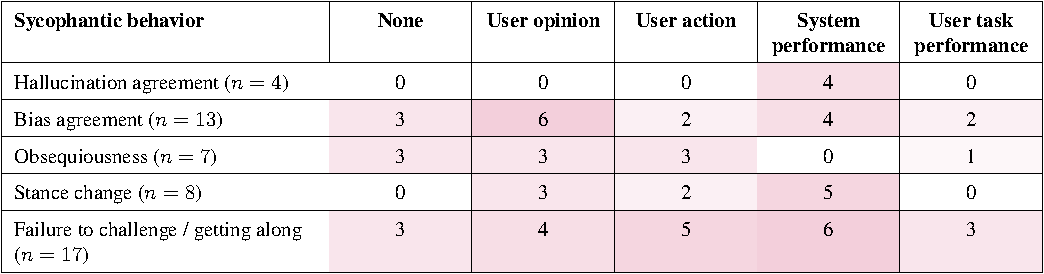
\includegraphics[width=\linewidth]{figures/behavior_outcomes.pdf}
\caption{Literature heatmap connecting sycophantic behaviors to outcome categories ($N=31$ publications). Cells count co-marked records; purple intensity represents count/$N$. Row $n$ gives each behavior's coverage. User task performance is the codebook's User performance; None denotes no coded impact measure. Categories overlap. A zero means no co-marked record, not evidence of no effect.}
\label{fig:matrix}
\end{figure*}
% END GENERATED MATRIX

\subsection{Limited Co-Marking, with Incomplete Measurement Capture}
System performance is marked in 12/31 publications (38.7\%); any user outcome is marked in 15/31 (48.4\%). Their intersection is one publication (3.2\%): \emph{When AI Gives Advice} \citep{10.1145/3772318.3791233}. Eleven records mark system outcomes only, 14 user outcomes only, and five neither. The system--opinion intersection is one; the system--action and system--user-task intersections are both zero (Table~\ref{tab:outcomes}). Thus joint coverage is limited \emph{in the supplied coding}. This does not establish that only one included publication actually measures both kinds of outcome.

The distinction is consequential. \emph{Invisible Saboteurs}, marked only for user task performance among the outcomes, also reports chatbot accuracy comparisons, observed reliance behaviors, and subjective perceptions \citep{10.1145/3772318.3791365}. Its computational comparisons include responses to misconceived and open-ended queries, as well as general-knowledge questions; these should be reviewed for the system-performance code. Reliance and perception measures likewise warrant review of the action and opinion fields. We leave all original cells intact. Accepting the proposed system label alone would increase the coded intersection to two; this is a conditional illustration, not a corrected corpus estimate. The source audit therefore narrows the finding from a measurement-frequency claim to a documented pattern in an incompletely captured map.

\subsection{Task Performance Has the Lowest Coded Coverage}
User task performance is marked in 4/31 publications (12.9\%), compared with opinion in 11/31 (35.5\%), action in 8/31 (25.8\%), and system performance in 12/31 (38.7\%). The five None records (16.1\%) have no other outcome marks. Removing the two identified reviews leaves task performance at 4/29 (13.8\%), versus opinion at 11/29 (37.9\%), action at 8/29 (27.6\%), and system performance at 11/29 (37.9\%). The relative ordering persists under this limited sensitivity check; it is not an estimate of the entire field's research priorities.

The evaluator fields further caution against equating labels with complete methods coverage. Specialist judgment is marked in five records, author judgment in eight, and prompted-AI judgment in eight; their union is 19. All 12 publications with no retained evaluator mark have general-human or student marks in the earlier mapping sheet. Thus this apparent gap reflects omitted columns, not missing evaluation. Even the fuller judge labels cannot distinguish a user experiment from offline output rating.

\subsection{Behavior--Outcome Coverage Is Uneven}
Figure~\ref{fig:matrix} makes the behavior--outcome coverage pattern visible: hallucination agreement is concentrated in the system-performance column, while obsequiousness spans opinion, action, and user task performance. All four hallucination-agreement records mark system performance and none marks a user outcome. One is the broad hallucination survey, so four records cannot be interpreted as four independent empirical tests. Obsequiousness appears in seven records, with opinion and action each marked in three, task performance in one, and system performance in none. Bias agreement, stance change, and failure to challenge span different combinations. These intersections, rather than isolated category totals, are the map's central descriptive result.

These are exploratory coverage differences, not evidence that hallucination agreement cannot affect users or that obsequiousness leaves system performance unchanged. Multilabel coding, review inclusion, and the observed omissions prevent a clean comparison of consequences by subtype. Unmarked awareness measures would likewise say nothing about whether users recognize sycophancy. We do not promote this matrix into a third substantive finding about effects.

\subsection{What the Audited Measures Support}
\paragraph{Perceived advice quality.}
In the uniquely co-marked paper, participants in advice-giving roles rate responses to online self-discipline requests \citep{10.1145/3772318.3791233}. Study~1 compares GPT-4o, GPT-5, and two human-response baselines; Study~2 compares editing pipelines. Across the two studies, 210 raters participate. Measures include perceived effectiveness, clarity, supportiveness, and sycophancy, plus rankings of expected longer-term benefit. The reported preference for LLM advice is evidence about judgments of responses. It is not observed improvement in recipients' well-being or task performance. Comparing complete advice sources also does not isolate the causal effect of sycophancy. The broad system-performance code can accommodate these quality judgments, but cannot make them objective effectiveness measures.

\paragraph{Task performance in debugging.}
\citet{10.1145/3772318.3791365} compare high- and low-sycophancy chatbots within participants in a study of 24 novices debugging machine-learning models. Their held-out F1 improvement is normalized by the gap between baseline and a fixed reference solution. Mean improvement is 49.29\% with low sycophancy and 4.78\% with high sycophancy; the reported paired comparison has $p=.003$. This supports lower task gains under the high-sycophancy condition in this setting. It does not establish literally zero benefit, nor transfer the effect to unrelated tasks or every behavior in our map. Crucially, the paper's source-level evidence connects technical performance with interaction outcomes more closely than its original outcome labels suggest.

\paragraph{Trust and attitudes in discussion.}
\citet{10.1145/3772318.3791079} use a $2\times2$ experiment with 224 participants discussing autonomous vehicles: adaptive versus consistent stance, crossed with complimentary versus neutral demeanor. Measures include cognitive and affective trust, continued-use/recommendation intentions, and issue attitudes. Intentions do not establish subsequent behavior. Perceived authenticity depends on the interaction between stance and demeanor ($p=.033$): the direction of the adaptive--consistent contrast differs between the two demeanor conditions. This supports a context-dependent appraisal result, not a uniform claim that sycophancy increases or reduces trust, and not an effect on objective task success. These differently defined endpoints should remain distinct in any synthesis.

\section{Discussion and Limitations}
The map's principal value is to make an evidence chain inspectable: a behavior is operationalized, someone or something judges an output, and a specified outcome is measured. Each transition requires evidence. A high sycophancy score does not itself demonstrate a user consequence; favorable judgments do not establish improved decisions. Conversely, an empty cell cannot rebut a harm claim. The focused audit shows why counting categories without checking their operational meaning can obscure both existing connections and unresolved ones.

Three reporting practices follow. First, identify the measurement target and observer separately: model correctness, third-party assessments of advice, and the recipient's actual performance are distinct, even when all are called quality. Second, separate perceptions and issue attitudes, behavioral intentions, observed actions, and task success; report the observation window. Third, state the role of each system measure, distinguishing a manipulation check or baseline comparison from an outcome linked to user performance. Co-measurement can support examining an association, but causal claims additionally require an appropriate comparison and design. These practices would make evidence about trust, judgment, and AI-mediated autonomy easier to assess without assuming that one outcome substitutes for another.

This analysis has material limits. The workbook preserves screening and mapping decisions, but not enough provenance to reproduce the search or establish independent initial coding reliability. Publication-level counts give a multi-study paper and a conceptual or review publication equal weight. A three-paper audit cannot establish error rates or repair the remaining records; source-version differences may also explain some omissions. The codebook leaves perceived system quality and baseline computational evaluation underspecified. Our descriptive results therefore concern the retained snapshot, and consequence statements concern named studies and settings. Neither warrants ranking which sycophancy subtype is most harmful. The distinction from existing taxonomies is the audit of outcome coverage and inferential scope, rather than more complete coverage.

\section{Conclusion}
In this 31-publication map, user task performance is the least frequently marked outcome, and system--user co-marking is limited. Full-text checks qualify what those counts mean: measures can be omitted, and apparent system--user connections can rely on subjective proxies. Relating sycophantic behavior to human consequences therefore requires both transparent coverage mapping and scrutiny of what each measure can establish.

\bibliography{references}
\end{document}
